%\documentclass{book}
%\begin{document}
\chapter{Introduction}
\lhead{Chapter 1. \emph{Introduction}}
Knowledge Discovery in Databases (KDD) is one of the most recent and interesting fields of research. Knowledge discovery in databases (KDD) has been created to identify efficient, helpful and valuable information from extreme large databases. The main goal of this field is to find the frequent, interesting and functional information from extremely large databases and use extract valuable information in different applications and research work. Discovered Knowledge can then be used to provide automated analysis and solutions to business. It has attracted a significant amount of research. In this KDD process, the result of data mining process is to find interesting, significant and useful patterns from massive data. In recent years, with increasing of modern technologies and huge use of internet there a lot of data is being produced. Extraction of important and significant patterns from this extreme large data repository and data sources is not that much easy. Moreover. relating these interesting patterns in real-life scenario is also very tough. The mining of useful and important information refers to the acquisition of previously unknown knowledge (e.g. frequent item-set) from extremely large data collections. Data mining is defined as a process of discovering important, potentially useful and valuable patterns from extremely large volumes of data. In finding interesting and significant relations, support is used as an indicator to find out if the pattern is interesting or not. The term Data Mining or Knowledge Discovery in Databases have been adopted for a field of research dealing with the automatic discovery of implicit information or knowledge within databases. In figure [~\ref{figure:dm_flow}] shows knowledge discovery process from extremely large data set. After mining process, some evaluation process runs to find the valuable information found from data mining process.\\
\begin{figure}
\centering
  \includegraphics[width=.9\textwidth]{images/dm_flow.jpg}
\caption{Knowledge Discovery Process}
\label{figure:dm_flow}
\end{figure}
Data mining is generally utilized by organizations (e.g., financial, retail, marketing and communication organizations) with a strong consumer focus. Found knowledge from mining result of can be used to relating association rules between objects, incidents, processes, finding the actual and correct strategy to C2C (consumer to consumer) marketing, B2B (business to business) marketing, B2C (business to consumer) marketing, and other marketing policy determination etc. In telecommunication industry, finding interesting valuable patterns for multidimensional analysis of telecommunication data, fraudulent pattern analysis, unusual patterns identification, and mobile telecommunication services the pattern mining helps a lot. In the medical science, semantic integration of heterogeneous, distributed genomic and proteomic databases, alignment, indexing, similarity search and comparative analysis, multiple nucleotide sequences, pattern mining in KDD process is very helpful. Moreover, in data warehouses, for data pre-processing and different data visualization this data mining process is very useful. In genetic algorithm analysis and finding characteristic of human, frequent pattern mining process is used. Discovery of structural patterns, analysis of genetic networks and protein pathways, association and path analysis, visualization tools in genetic data analysis, data mining is very much effectively used process.


\section{Frequent Pattern Mining}
\begin{figure}
\centering
  \includegraphics[width=.9\textwidth]{images/mining_class.jpg}
\caption{Data Mining Areas}
\label{figure:mining_class}
\end{figure}
In knowledge discovery process, finding frequent item-sets, sequences, sub-sequences, structures or other substructures are the usually first step to analyze a big-scale dataset. This frequent pattern mining has been one of the most recent, interesting and focused topic for researchers. Finding frequent item-set is first major challenges for researchers. As shown in ~\cite{apriori}, the real-life data sources are surprising that much large that cannot be thought to be stored in the single database and that causes the main challenges to find frequent patterns. For finding knowledge from these extremely large and un-grouped data sources first step is to find frequent item-sets. Frequent item-sets can be referred to a group of items those are frequent (with respect to minimum value predefined earlier) among the databases. If an item-set contains \emph{k} items, that can be called \emph{k-item-set}. For example, let an item-set \{iPhone, Head Phone\}. As the item-set contains 2 items, then it is \emph{2-item-set}. In a transaction DB the number of times item-set exists is called its support. The number of transactions required for the item-set to satisfy minimum support is therefore referred to as the minimum support count. Item-sets satisfy minimum support count value is treated as frequent item-set. For example, if {iPhone, Head Phone} exists in a transaction DB for 5 times and minimum support count threshold is 4 than item-set {iPhone, Head Phone} is treated as frequent item-set. If it is less than 4 then it can be treated as infrequent.\\
In data mining domain, one of the most significant and interesting, important area is frequent item-set finding (figure-~\ref{figure:mining_class}). A frequent item-set is very much valuable as always we need to find the relation between items then the first step is to find the frequency and the most frequent item-set has the high probability to be valuable. Moreover association rule mining, prediction, correlation mining, classification and other important evaluation need to first find frequent patterns. The frequent item-set finding is named as frequent pattern mining in term of KDD process.\\
\begin{figure}
\centering
  \includegraphics[width=.9\textwidth]{images/frequent_flow.jpg}
\caption{Frequent Pattern Mining Process}
\label{figure:frequent_flow}
\end{figure}
Many approaches have been developed and proposed for finding frequent item-sets in large data base. Apriori ~\cite{apriori} is the one of the major approaches that have been proposed two decades ago. FP-growth ~\cite{fp_growth} is the first tree structure based approach for finding such frequent patterns. For sequential item-set mining GSP ~\cite{gsp} , Prefix-Span ~\cite{prefix_span}, for closed pattern mining CLOSET ~\cite{closet}, CLOSET$+$ ~\cite{closet_plus}, CHARM ~\cite{charm}, TPF ~\cite{tpf}, others (~\cite{close_1}, ~\cite{close_2}) , for high utility pattern mining HUP-mining ~\cite{hup_mining}, for association rule mining ~\cite{ass_01}, ~\cite{ass_02}, ~\cite{ass_03}, ~\cite{ass_04}, ~\cite{ass_05}, ~\cite{ass_06}, ~\cite{ass_07}, constrain based pattern mining ~\cite{const_01} was proposed. In each of the approach item-set having support greater or equal to minimum support threshold is treated as frequent item-set.

\subsection{Uncertain Data}
\begin{figure}
\centering
  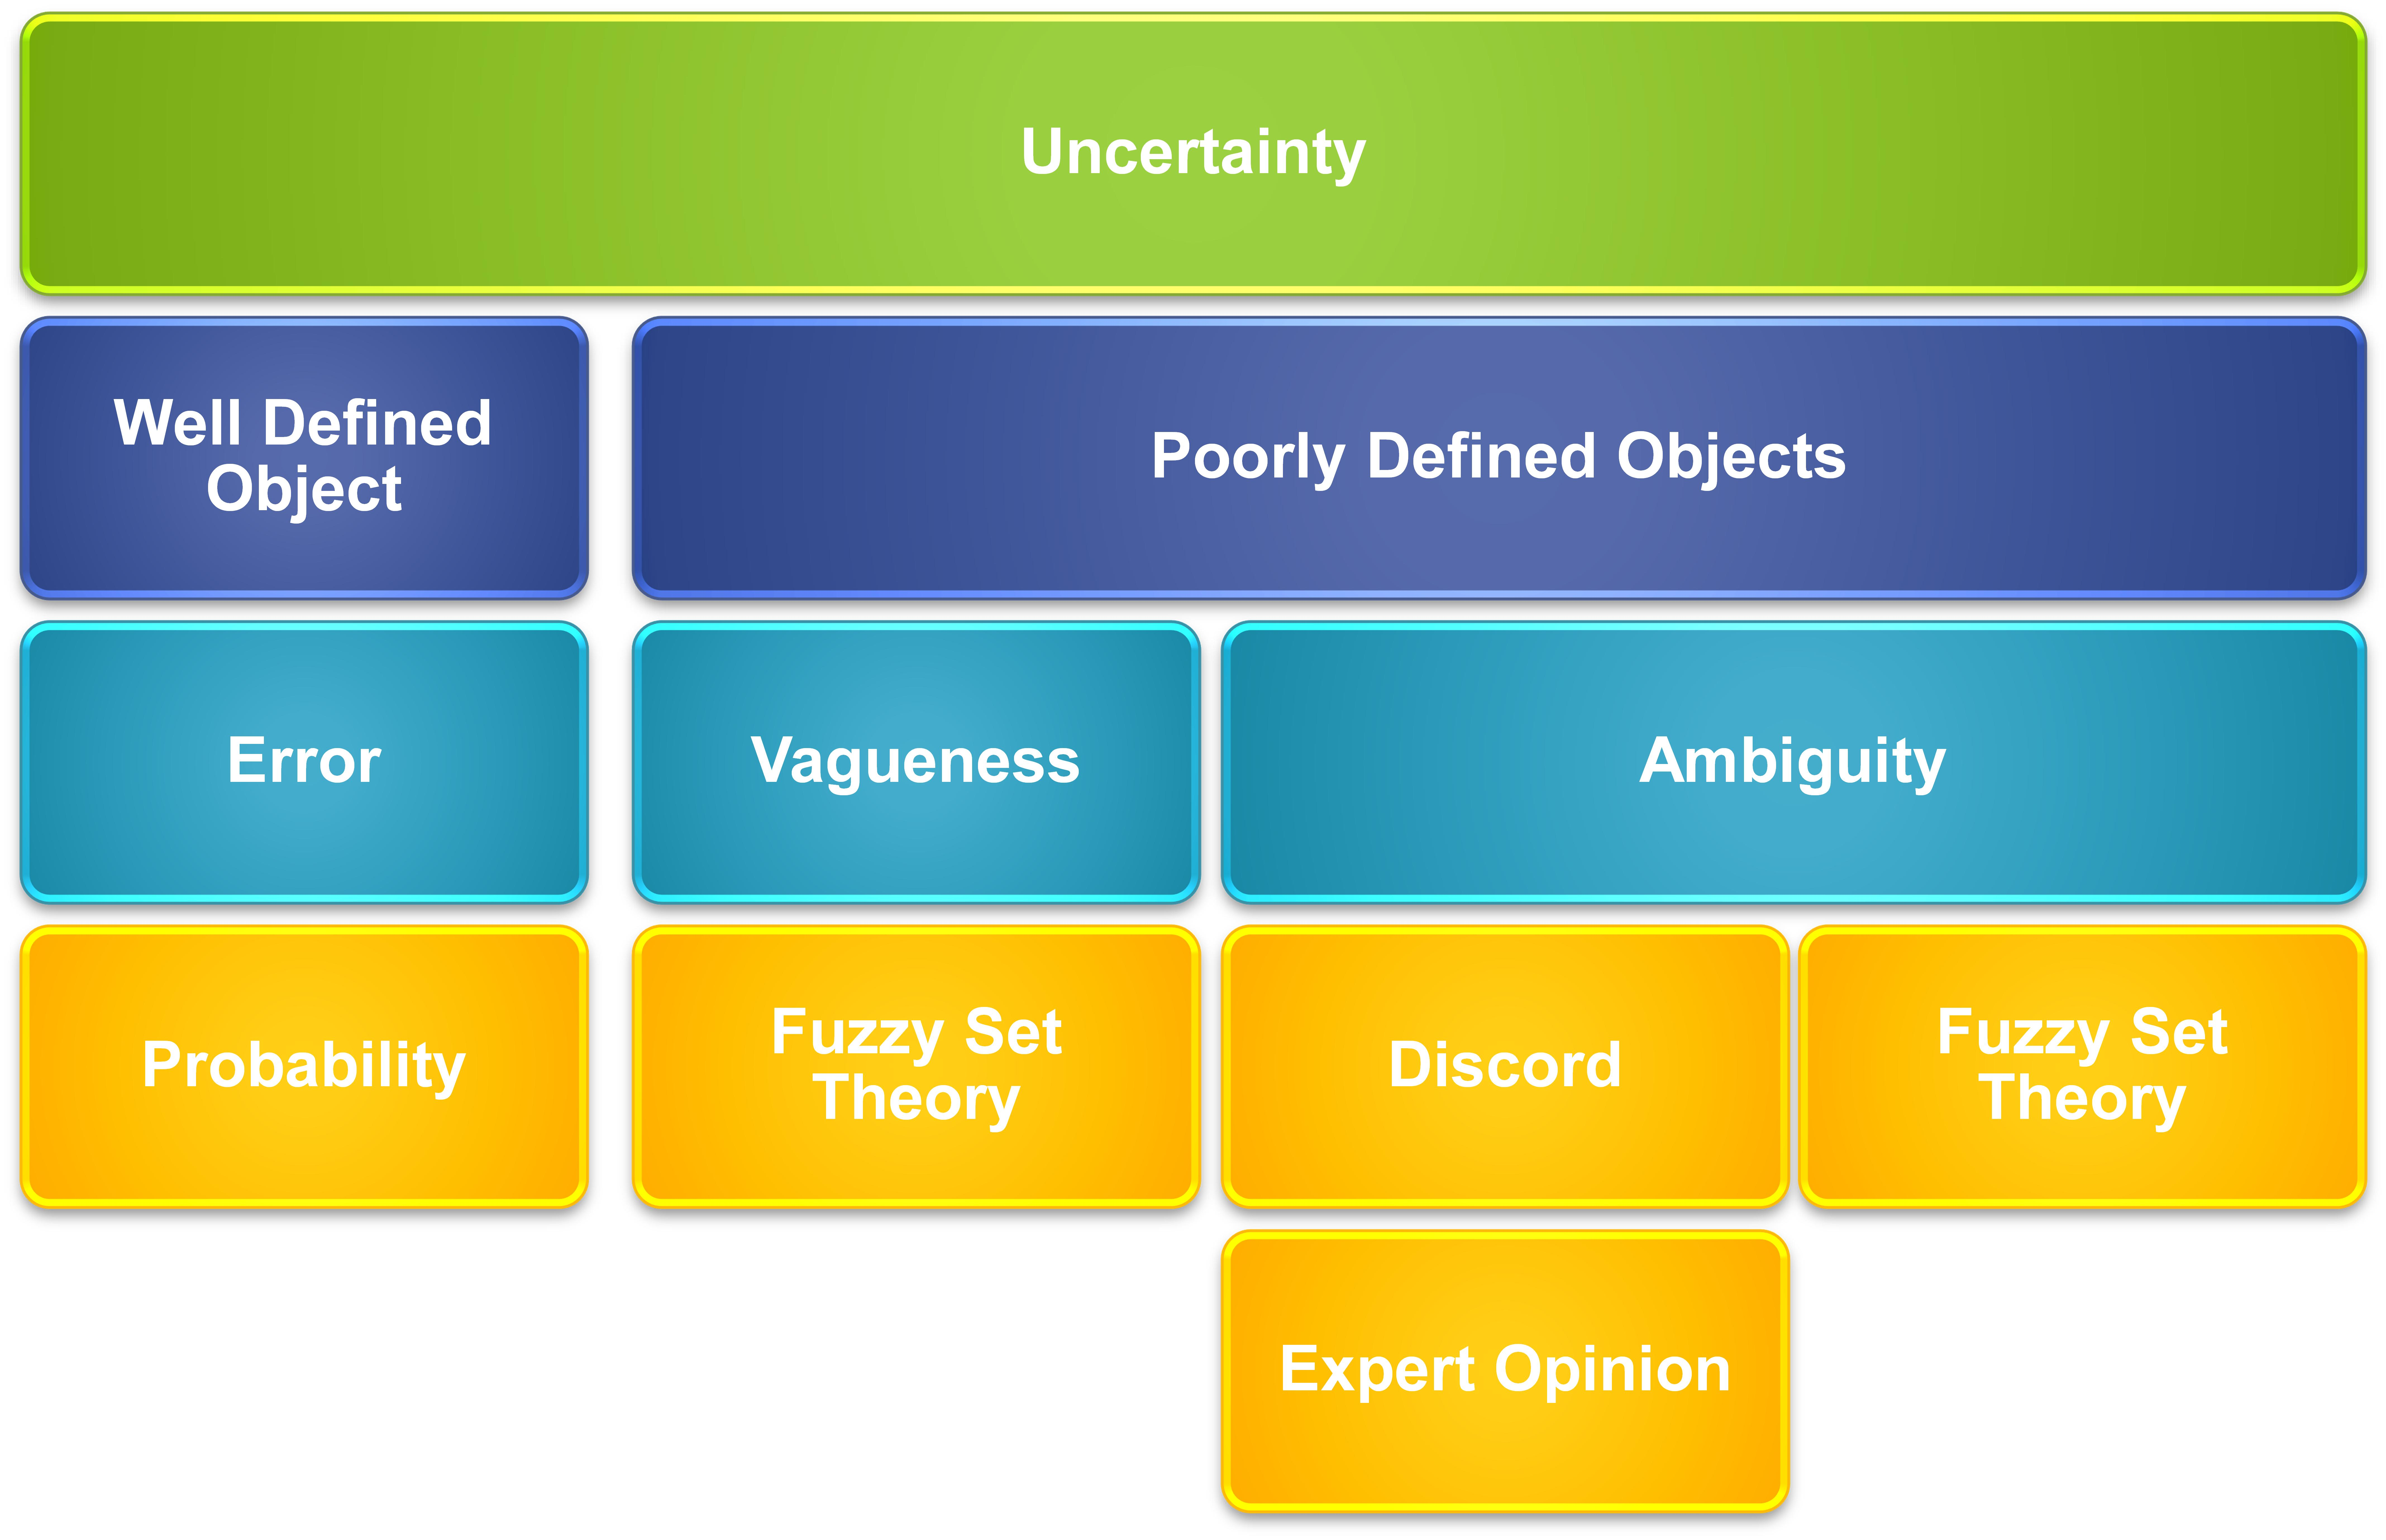
\includegraphics[width=.9\textwidth]{images/uncertainity_type.jpg}
\caption{Types of Uncertainty}
\label{figure:uncertainity_type}
\end{figure}
Real-life data analysis shows that the real-life data sources do not produce always certain data. Many real-life data source produces data with error (correctness is not certain). These types of data are named as uncertain data. Figure \ref{figure:uncertainity_type} shows the uncertainty types of real-life dataset. For example location data from GPS sensors mostly produces erroneous data. The correctness of the data is always uncertain. For the uncertainty specialty, these types of data get special attention and concerns to work with. Normal support count is not possible in this type of dataset. This type of database contains data with their corresponding existential probability. Frequent pattern mining of this type of data very much harder. For example, a physician may highly suspicious (but cannot guarantee) that a patient suffers from flu if the patient comes to him having the high fever. The uncertainty of such prediction can be expressed in terms of existential probability. For instance, a patient may have a 90\% likelihood of having the flu, and a 20\% likelihood of having a cold regardless of having the flu. So the probability of having the flu is 0.80 and the probability of having a cold is 0.20. So many real-life dataset may be in between existence and nonexistence. In these situation, an item-set \emph{a\textsubscript{i}} can have own existential probability in \emph{a\textsubscript{i}} between 0 and 1 ($P_i (0 < P_i < 1)$). Actually understanding uncertain data is the very much tough task but really uncertain data exists everywhere. They come with uncertainty to make us confused in terms of poorly defined object, fuzzy sets, ambiguity, error, inherent probability etc. (Figure \ref{figure:uncertainity_type}).\\
There are much real-life scenarios where data source always come with uncertainty. Information gathered from World Wide Web always inherits uncertainty. For example, a system is monitoring user behavior in World Wide Web. It collects data from different websites, extract information and analyze. After the certain period, it finds that one user Mr. X is the citizen of country Y. As he/she can work in Y, there must be a probability that Mr. X is the citizen of Y. There must be a probability value associated with Mr. X's citizenship. So the data is definitely uncertain. Many sensors produce values with some error like 10\% error from GPS data or temperature reading from cell phones.\\
Many approaches have been introduced for finding frequent patterns over uncertain data (U-Apriori ~\cite{u_priori}, UF-growth ~\cite{uf_growth}, UFP-growth ~\cite{ufp_growth} etc.). As the data existence in the database is not certain then normal support calculation is not easy that makes uncertain data very mysterious. So exact frequent pattern finding makes a huge resource sacrifice. For the improvement many approximate algorithms have been proposed (CUF-growth ~\cite{cuf_growth}, CUF\textsuperscript{*}-growth ~\cite{cuf_growth}, PUF-growth ~\cite{puf_growth}). Most of them suffer producing false positives. False positives are those which are not actually frequent but exist in frequent pattern set.

\subsection{Stream Data}
In real-life with the enormous use of the internet, artificial computerized and artificially intelligent devices (smartphones, tablet PC, cars, smart cards etc.) the data source produces a stream millions of data each and every micro second. Storing these data in some storage is out of think nowadays. But this huge data is very valuable for getting interesting information. Moreover, once these data flooded away then can never be found again. The most important property of this kind of dataset is this dataset is unbounded and restless and cannot be defined previously, how much data will come in future. Most recent data is most important but old one is not insignificant and cannot be ignored. This produces a great challenge for researchers to find interesting information from a continuous data stream.\\
For example with the growth of smartphone users much more applications are hitting each and every second. From these usages and data flood finding user behavior to offer some promotional offer for increasing the sale of the online retailer is the very tough job. Another example can be the CCTV video footage of traffic camera. That produces a large number of data flood. In this regard, any sort of any terrorist activity prediction will be very much significant and necessary information for the government. But for a lot of continuous data makes this a very hard job.\\
Stream data makes the database dynamic as there is no limit of data. To find frequent item-set in data stream several algorithms (~\cite{uncertain_01}, ~\cite{uncertain_02}, ~\cite{uncertain_03}, ~\cite{uncertain_04}, ~\cite{uncertain_05}, ~\cite{uncertain_06}) have been proposed. But most are for handling stream but certain data. The uncertainty property makes mining task more complex and complicated the data stream. FP-streaming ~\cite{suf_growth} and SUF-growth ~\cite{suf_growth} have been proposed for finding frequent, interesting patterns from uncertain and stream data. But these approaches have to compromise runtime efficiency or correctness. However these SUF-growth ~\cite{suf_growth} is an exact approach to finding frequent patterns.
\begin{figure}
\centering
  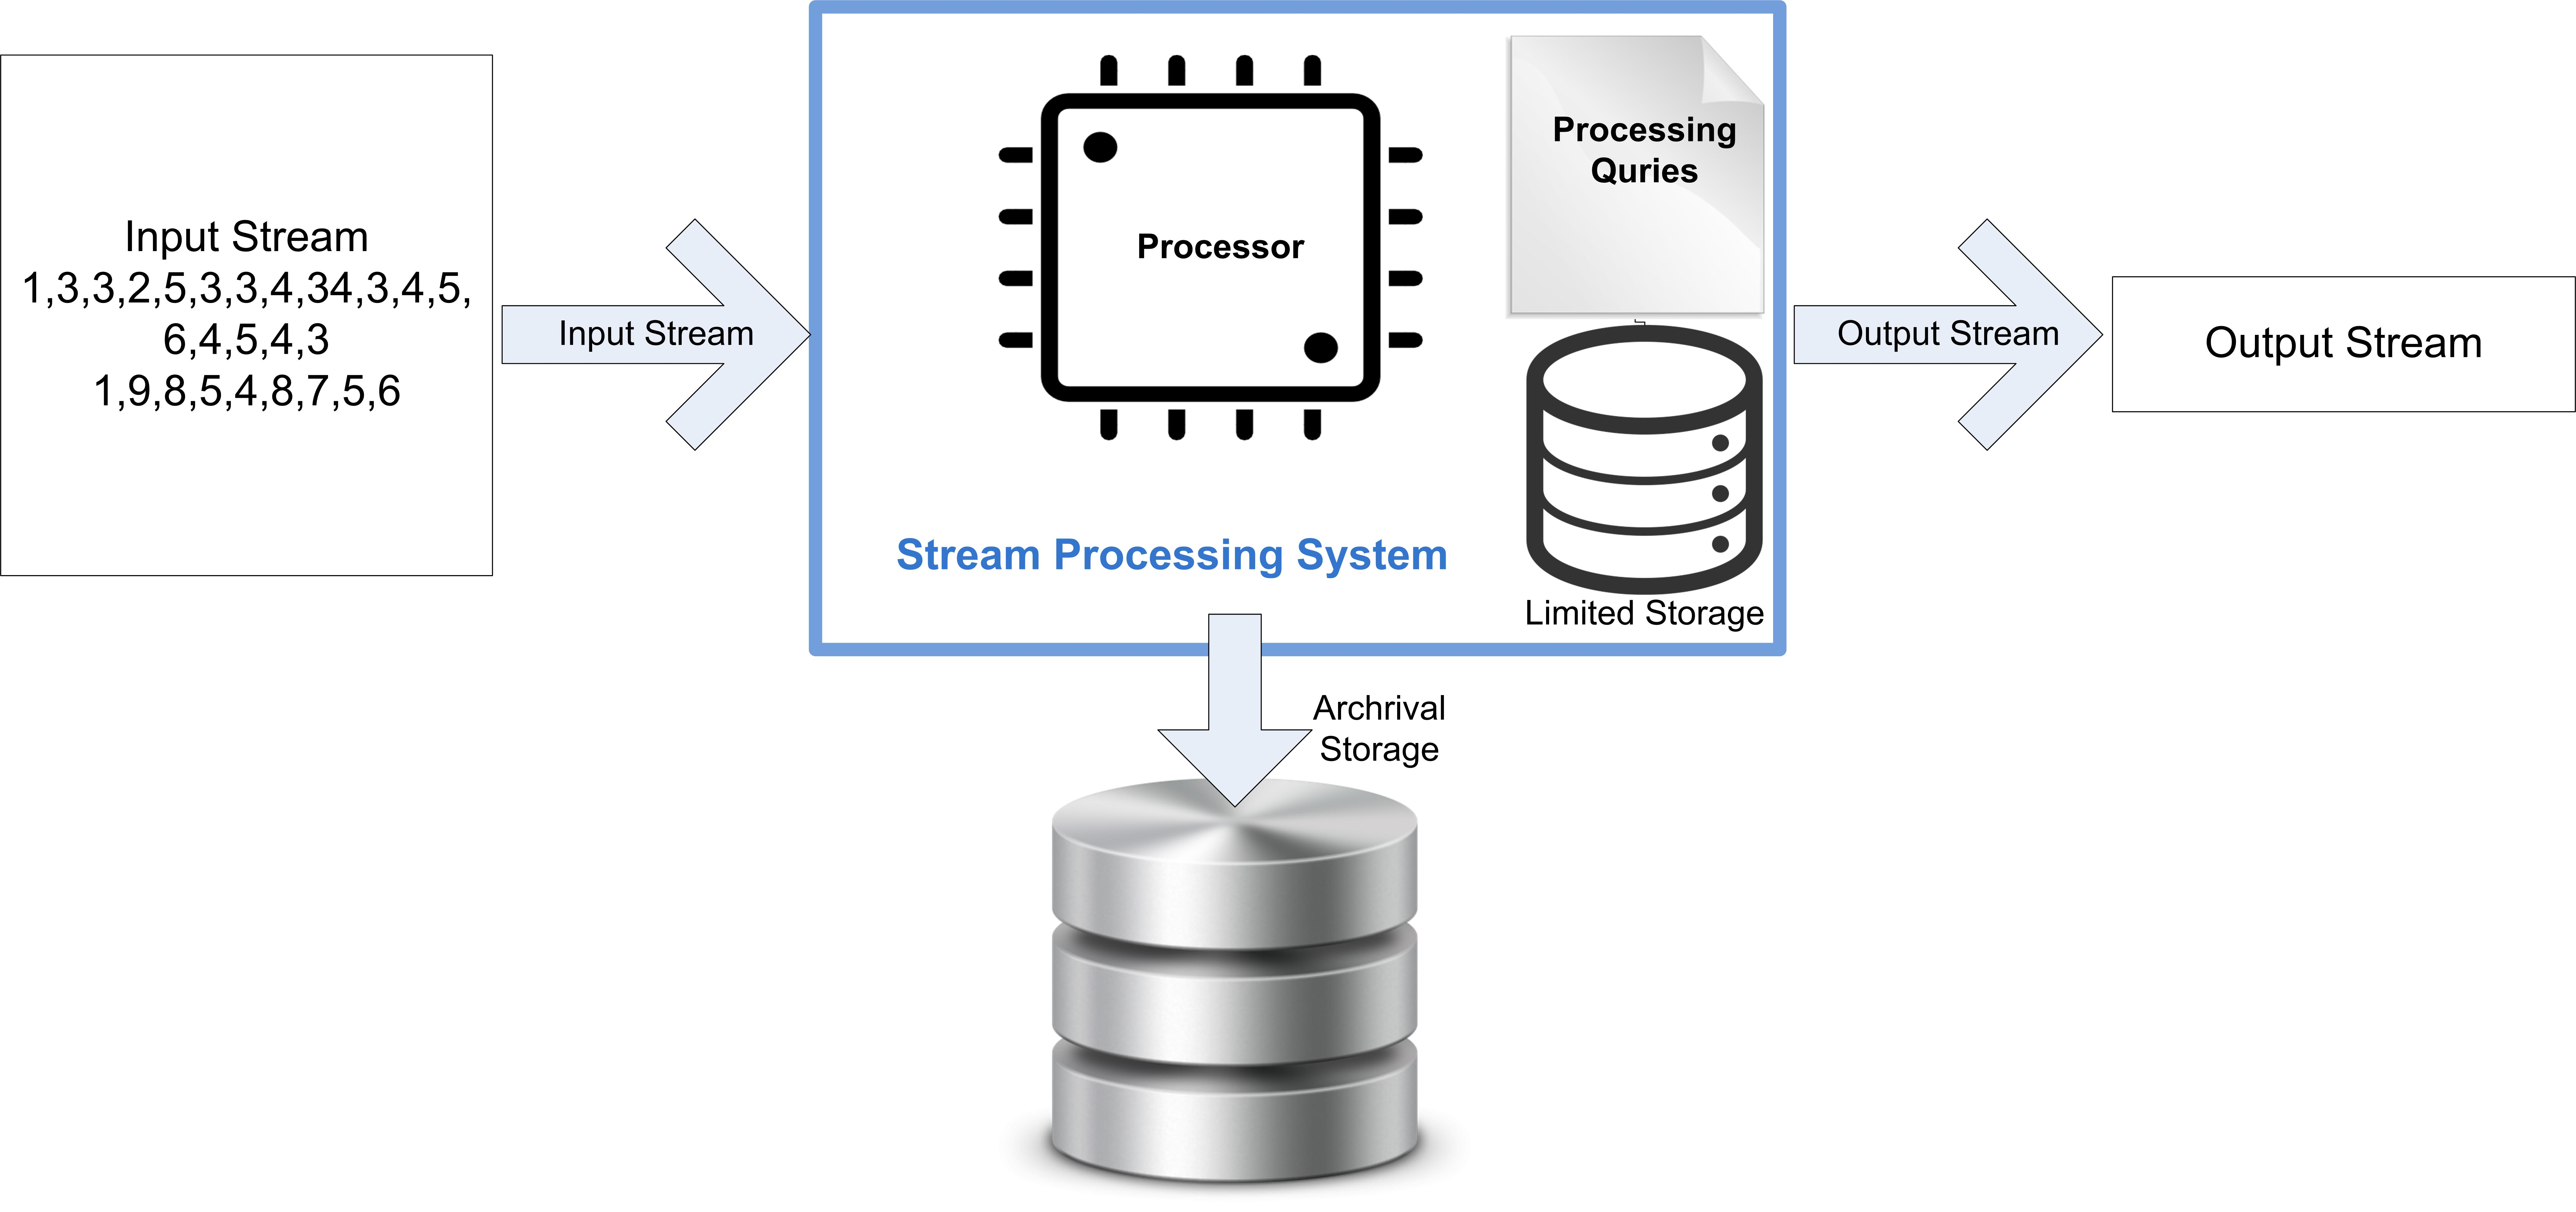
\includegraphics[width=.9\textwidth]{images/stream_data.jpg}
\caption{Stream Processing Steps}
\label{figure:stream_data}
\end{figure}


\section{Motivating Example}
Let us consider \emph{Google Search} ~\cite{google} service as our data source. If we analyze the data coming from source, we find that in each and every millisecond, thousands of people and intelligent devices (e.g. different smart applications of smartphones or PC) are searching in \emph{Google Search}. This search is a continuous process and never stops and we cannot predict earlier when the incoming will be fast and when it will be slow. We can think data incoming like stream. Now if we look at search criteria, we find that \emph{Google Search} service users (both human and machine) are not always searching exactly what she/he/it is looking for. There is much more search with partial key data or key words. For example, when a user searches in Google with key word \emph{Tom Cruise} we cannot surely tell that she/he/it wants to get information of personal life of \emph{Tom Cruise}, next up-coming movie, his movie list, awards he already got or his social activities. We can hardly say, if he is searching for Hollywood movie actor or any other person. This fact makes the task very difficult to find the exact intention of user. The search information is with noise and we do not know exactly that the search key word is with noise or not. So the found information from the \emph{Google Search} is uncertain. The whole scenario indicates to uncertain stream data. \\
Now, if we want to find frequent searched patterns from \emph{Google Search} data then we have to find frequent patterns from these uncertain stream data. Now how can these patterns make us interested, is the first and foremost important question. Let’s consider, after finding frequent patterns, we get information that people are searching for baby food, baby wear for heavy winter, child specialist doctor etc. then we get many important decision. For online retailers the message can be such that if they discount on different products used by babies will increase their sale. For government, now this is heavy winter and much more children are being sick and need to take concerns. This information is really very much valuable.\\
From this scenario it is clear that the gathered information form \emph{Google Search} is very much dynamic and people search criteria can be changed without any prediction and this criteria is always dynamic that makes the frequent patterns finding form found information very much difficult. Again keeping all search information is very much costly as lots of incoming data flow is coming each time. Moreover, the incoming data is not that much precise that we can get any direct conclusion from the search key words.
\section{Objectives}
Many algorithms and approaches have been proposed for mining frequent patterns over certain and uncertain data. Among them in uncertain data mining, exact approaches suffer from runtime optimization problem. The probabilistic model based approaches suffer from either huge false positives or false negative generation problem. Moreover, extraction knowledge from stream data is another challenge. It is one of the newest topics for researchers. The findings of challenges and difficulties of finding frequent item-set form uncertain data are given:
\begin{itemize}
    \item Existing algorithms for uncertain data mining suffers either from runtime compromise or the compactness of data structure.
    \item Probabilistic uncertain data modeling approach suffers from huge false positives or false negative with the frequent item-set.
    \item The proposed data structure in existing approaches for mining uncertain stream data suffers from memory optimization.
    \item Reduction of huge false positives or false negatives from candidate frequent item-set suffers from runtime inefficiency.
\end{itemize}
To overcome these problems we have followed some objectives. They are given below:
\begin{itemize}
    \item A completely new, correct, efficient, robust, scalable and exact approach, with the new data structure, that will memory efficient.
    \item Design and propose a new memory and runtime efficient data-structure, which will work for both uncertain dynamic database and static databases.
    \item Attach any meta-data with each item of transaction that will make the runtime storage compact as much as possible.
    \item Most recent data is more significant - with this characteristic storing as much as recent data that has more probability to be important.
   \item Giving user the opportunity to keep her/his recent information, she/he wishes. 
\end{itemize}

\section{Our Contribution}
Our key contributions of this paper are given below:
\begin{itemize}
	\item We have introduced a prefix value, \emph{U\textsuperscript{cap}} for each item in a transaction which always maintains upper bound of probability. That helps us to make compact pattern tree construction.
	\item A new data-structure \emph{US-tree}, that is very much compact and very memory efficient.
	\item Propose a data-structure will follow the partial downward closure property.
	\item A new mining algorithm \emph{USFP-growth} algorithm, that will reduce mining time surprisingly.
	\item Propose an approach, which will both runtime and memory efficient, scalable and will have wide range of applicable area.
	\end{itemize}
\section{Thesis Organization}
	We have carried out the thesis work to consummate the objectives. An outline of rest of the chapters is provided as follows:
	\paragraph{Chapter 2} describes the necessary background studies and existing approaches.
	\paragraph{Chapter 3} provides the details of our proposed approach with required analysis.
	\paragraph{Chapter 4} presents the results of experimental results in detail with comparison and analysis.
	\paragraph{Chapter 5} ends the thesis with a brief conclusion and future scopes.
%\end{document}
